\section{Open points and information}
\label{sec:open_points}
\label{hints}

This chapter regroups some points that are still open and some useful information for taking decisions about the future step to do in the ViSaG project. Some of those points have been discussed and a decision has been made (see Chapter \ref{weakness} for the decisions made). 

\subsection{VMware VIX API}
VMware provides a C based API to interact with VM. This API has some interesting function that could help us in the development of the Virtual version of POP-C++. These functions are: 

\begin{itemize}
\item \textbf{VixVM\_Clone} : cloning an existent VM with snapshot (unimplemented with ESXi).
\item \textbf{VixVM\_CopyFileFromGuestToHost} : copy a file from the guest VM (worker) to the host VM (admin)
\item \textbf{VixVM\_CopyFileFromHostToGuest} : copy a file from the host VM (admin) to the guest VM (worker)
\item \textbf{VixVM\_ReadVariable} : some property of the VM (ip address) could be read like that.
\end{itemize}

The VIX 1.10 API reference can be found at following URL: \\
http://www.vmware.com/support/developer/vix-api/vix110\_reference/\s

\textit{NOTE:} The "product support" section of the reference cited above mentions that the function VixVM\_Clone is only supported on VMware Workstation platform.\s

\textit{REMARK:} Using a proprietary API could be a little bit restrictive but it would also be much more reliable than the use of command line tools that are also proprietary.

\subsection{Cloning}
The cloning process of a VM is going like this : 

\begin{enumerate}
\item Create a new folder on the data store (vifs --mkdir).
\item Copy every files from the original VM folder to the new folder (except log files) (vmkfstools -i).
\item Modify the "display name" of the VM (vifs -g, awk, vifs -p).
\item Register the new VM in the inventory (vmware-cmd).
\item Start the VM (vmware-cmd).
\end{enumerate}

This solution could be easily implemented in the current version of Virtual POP-C++ (a shell script is already working for that purpose). \s

\textit{NOTE(1):} None of the VIX API or LIBVIRT is able to provide this function for the moment. \s

\textit{NOTE(2):} When a worker is cloned, the SSH pairs is the same on the original VM and on the cloned VM. This is not a problem for the functionality of POP-C++. It could be a bad practice from a security point of view. We could force the worker to generate new key after the cloning process by launching a command with VIX.  

\subsection{Key exchange with the VM}
The workerDeamon must be changed because now it is not reliable and not secure enough. In addition, with the secure version, the worker VM must be able to do more than just receive a key.  Here are the needs for the key exchange:

\begin{itemize}
\item The admin must be able to read the PKI of the worker.
\item The worker must accept PKI from the admin.
\end{itemize}

The VIX API gives a way to copy a file from a host to a guest. This API also gives a way to execute a program on the guest.\s

\subsection{Names and addresses used in Virtual POP-C++}
POP-C++ and its virtual version use different mechanism to retrieve a machine identity. Here is a brief summary of methods used in the virtual version of POP-C++ currently in development.\s


\textbf{Between Global Services}\\
Between the global services, either the IP address or the hostname could be used. \s

\textbf{Between VM-admin and VM-worker}\\
Between the VM-admin and the VM-worker two different kind of identification are used. Firstly, when the admin reverts the worker to the correct snapshot, the "display name" of the VM is used. This "display name" is a notion from VMware ESXi. A VM is registered under this name in the vSphere inventory (see Figure \ref{fig:vsphere}). With this "display name", the admin is able to retrieve the IP address of the worker. Once the admin knows the worker IP address it can communicate directly with the worker (at this point the hostname could also be used). 

\begin{figure}[ht]
	\caption{vSphere Client - inventory (display name)}
  	\centering
	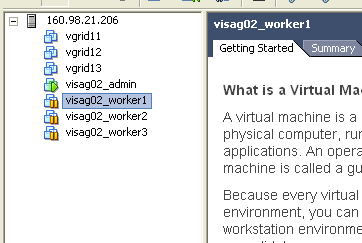
\includegraphics[scale=1.0]{../inventory.png}
	\label{fig:vsphere}
\end{figure}

\subsection{DHCP}
Using the DHCP service for the worker is not without any risks. This section will list the known issues about its usage. \s

\textbf{Lease on a suspended VM}\\
DHCP service uses lease for IP address. When a VM is reverted to a snapshot from a "shutdown state" or a "suspended state", the lease could be expired and the IP address may change after a few minutes. This behaviour could make the POP-C++ application crash. A solution to this problem is to force the VM to ask for a new lease when it is reverted. In this case the IP address would be changed before any execution on the worker and the application could run normally. 





